\section{Замеры}

\subsection{$U = 1$}
Для вычислений были сгенерированы по 1000 реплик длины 250, 500, 1000, 2000. При моделировании методом Монте-Карло делалось 10000--30000 шагов на отжиг, и 50000--100000 шагов для замеров. 
Оказалось что достаточно большая часть этих конформаций неплотные, то есть их свойства ближе к свойствам одномерной решётки, чем двумерной. При попытке посчитать среднее значения кумулянта Биндера неплотные конформации Сильно влияли на значение кумулянта, увеличивая погрешность от реплики к реплике.

\begin{figure}[h]
	\centering
	\begin{subfigure}[t]{0.48\textwidth}
		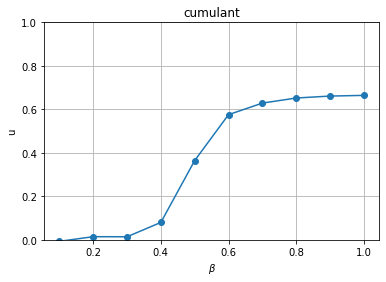
\includegraphics[width=\textwidth]{../images/dense_cumulant.png} 
		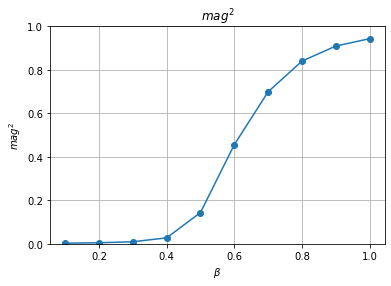
\includegraphics[width=\textwidth]{../images/dense_magnetization.png} 
		\caption{Плотная}
	\end{subfigure}
	\begin{subfigure}[t]{0.48\textwidth}
		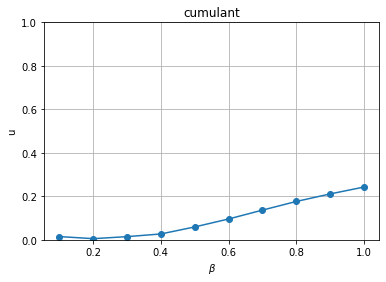
\includegraphics[width=\textwidth]{../images/loose_cumulant.png} 
		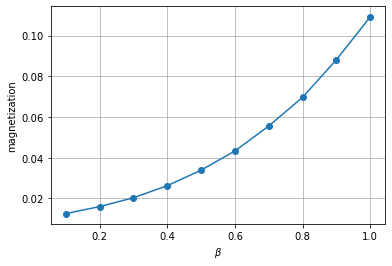
\includegraphics[width=\textwidth]{../images/loose_magnetization.png} 
		\caption{Неплотная}
	\end{subfigure}
	\caption{Пример кумулянта и намагниченности плотной и неплотной конформаций}
\end{figure}


\subsubsection{Разделение конформаций}

Для отделения плотных конформаций от остальных было предложено вычислять их радиус инерции.$R = \sqrt{\frac{1}{n}\sum_{i=1}^{n}r_{i}^{2}}$, где $r_i$ это расстояние от узла конформации до её центра масс. Однако при рассмотрении большого количества конформаций оказалось, что маленький радиус инерции не гарантирует хорошую намагниченность конформации. Это хорошо видно при рассмотрении намагниченности конформаций при низких температурах $\beta = 1$

\begin{figure}[h]
	\centering
	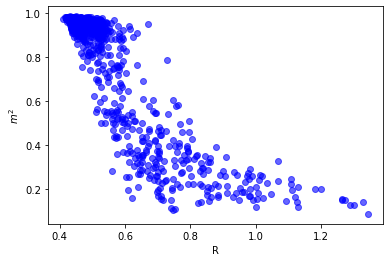
\includegraphics[width=\textwidth]{../images/mag2_to_R_L250.png} 
	\caption{Корреляция намагниченности конформаций при $\beta = 1$ и радиуса инерции для конформаций длины $L = 250$}
	\label{fig:mag2_to_R} 
\end{figure}

На рис.\ref{fig:mag2_to_R}, при $R \approx 0.6$ $m^2$ принимают любые значения от $0.2$ до $1.0$. Значит, при разделении конформации только по радиусу инерции, мы либо будем отбрасывать намагничивающиеся конформации, либо оставлять не намагничивающиеся

\paragraph{Кластеризованные конформации}

\begin{figure}[h!]
	\centering
	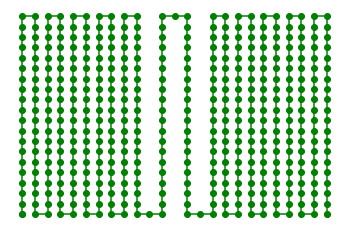
\includegraphics[width=0.47\textwidth]{../images/2Cluster_conformation.png}
	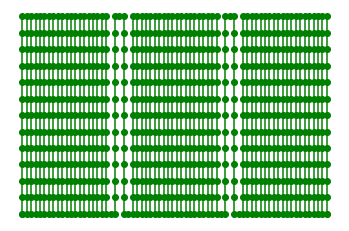
\includegraphics[width=0.47\textwidth]{../images/3Cluster_conformation.png} 
	\caption{Пример плотных немагнитных конформаций с двумя и тремя кластерами}
	\label{fig:synth_cluster_conf}
\end{figure}

На искусственном примере рис.\ref{fig:synth_cluster_conf} показана одна из причин, по которой плотная конформация может плохо намагничиваться. Тут имеется несколько крупных двумерных кластеров, соединённых одномерной цепочкой. И не смотря на то, что сами по себе эти кластеры намагничиваются, направление спинов в них слабо связано, из-за чего спины в разных кластерах с большой вероятностью будут направлены в противоположные стороны. Далее соединяющие цепочки будут называться мостами, длина моста - количество вершин, входящих в него.

На рис.\ref{fig:synth_cluster_conf} приведён пример с очень длинным мостом, чтобы показать, что длина моста почти не влияет на радиус инерции конформации. Однако даже в конформациях с короткими мостами можно наблюдать большую разницу в намагниченности по сравнению с конформациями без мостов (рис.\ref{fig:mag_from_bridge_length}). 

\begin{figure}[h!]
	\centering
	\begin{subfigure}[t]{0.4\textwidth} 
		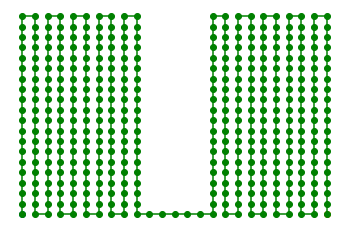
\includegraphics[width=\textwidth]{../images/2Cluster_conformation_short_link.png} 
		\caption{Приме с мостом длины 5}
	\end{subfigure} 
	\begin{subfigure}[t]{0.58\textwidth} 
		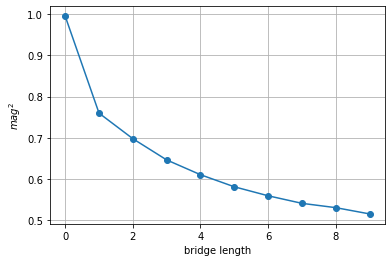
\includegraphics[width=\textwidth]{../images/mag2_from_bridge_length_in_two_clusters.png} 
		\caption{График зависимости намагниченности от длины моста}
	\end{subfigure} 
	\caption{Значения намагниченности для конформации с двумя кластерами при различных длинах моста. Длина 0 означает, что рассматривалась конформация без моста, состоящая из одного кластера.}
	\label{fig:mag_from_bridge_length}
\end{figure}

Было сделано предположение, что можно определять намагничивающиеся конформации используя кластеры и мосты. Следующей задачей стало проанализировать конформации на количество и размеры кластеров, а так же мостов. Однако пока мы не дали чёткого определения моста и кластера. Поэтому были рассмотрены несколько вариантов.

Первым вариантом было искать классические мосты -- спины, при удалении увеличивается число компонент связанности графа. Однако такой способ не дал желаемого эффекта, так как кластеры могут быть соединены более чем одним мостом. И например на конформации из рис. \ref{fig:clusters_and_bridges} данный способ не выделяет ни одного моста, хотя там очевидно есть структуры, отделённые друг от друга одномерными цепочками. 

Следующий алгоритм выделял как мосты все цепочки спинов у которых 1 или 2 соседа, однако при таком подходе мы получаем мосты, которые соединяют один и тот же кластер. Такие мосты не разделяют кластеры и не оказывают на конформацию эффект описанный выше. Так же этим способом мы выделяем множество вершин на краях конформации как мосты, например вершины в углах прямоугольника будут считаться мостами, что очевидно неправильно.

Итоговая версия алгоритма выделяет как мосты все спины, которые имеют 1 или 2 соседа, и затем добавляет мосты, которые соединяют один и тот же кластер, к этому же кластеру. Таким образом мы оставляем только мосты, которые разделяют конформацию на отдельные плотные части, которые мы и называем кластерами. Данный алгоритм описан ниже.

\paragraph{Алгоритм разбиения на мосты и кластеры}
\begin{enumerate}
	\item Отметить все спины с 1 или 2 соседями как мосты.
	\item Создаём массив, где отмечаем посещённые спины. Создаём массив где для каждого спина будем писать номер его кластера. И переменную отвечающую за текущую длину моста $l$. Изначально все спины не посещены, $l = 0$.
	\item Начинаем идти по конформации от первой вершины.
	\begin{enumerate}
	
		\item Если спин отмечен как мост, то увеличиваем $l$ на 1
		\item Если спин не отмечен как мост, и не посещён. Увеличиваем счётчик кластеров на 1 и запускаем DFS(Алгоритм DFS описан ниже). Если $l > 0$ увеличиваем счётчик мостов на 1, длина нового моста $= l$. Обнуляем $l$
		\item Если спин не мост, уже посещён, последний встреченный спин, не являющийся мостом, принадлежит тому же кластеру и текущая длина моста $l > 0$. Значит этот мост соединяет один и тот же кластер. Поэтому добавляем предыдущие $l$ спинов к этому кластеру, обнуляем $l$.
		\item Если спин не мост, посещён, но номер кластера отличается от последнего встреченного кластера. Если $l > 0$ увеличиваем счётчик мостов на 1, длина нового моста $= l$. Обнуляем $l$
	\end{enumerate}
	\item Проверяем первый и последний мост, если они соединяют один и тот же кластер, или один из их концов не соединён ни с каким кластером, добавляем их в кластер, с которым они соединены.
\end{enumerate}

\textbf{Алгоритм DFS}
\begin{enumerate}
	\item Заходим в вершину.
	\item Отмечаем вершину как посещённую.
	\item Отмечаем номер её кластера.
	\item Увеличиваем счётчик размера текущего кластера на 1.
	\item Заходим во все соседние не посещённые вершины не мосты.
\end{enumerate}

В данном алгоритме мы пользуемся тем, что мосты обязательно образуются из подряд идущих вершин конформации. Поэтому чтобы определить соединяет ли мост один и тот же кластер, нам достаточно, идя по конформации, запоминать последний встреченный кластер и сравнивать его с новым.

\begin{figure}[h]
	\centering
	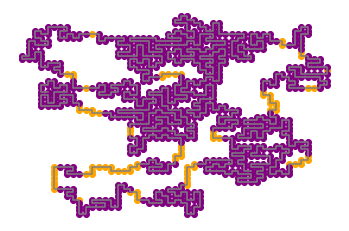
\includegraphics[width=0.70\textwidth]{../images/bridges_example_1.png}  
	\caption{Пример реальных конформаций с маленьким радиусом инерции и маленькой намагниченностью, с отмеченными мостами}
	\label{fig:clusters_and_bridges}
\end{figure}

\subsection{Статистика по кластерам и мостам}
Ниже представлены гистограммы с размерами и числом кластеров и мостов в конформациях. Посчитано на 10000 конформациях с длинами 250, 500, 10000, конформации получены при $\frac{U}{T} = 1$. Размеры кластеров и длины мостов нормированы на длины конформаций. 


\begin{figure}[H]
	\centering
	\begin{subfigure}[t]{0.3\textwidth} 
		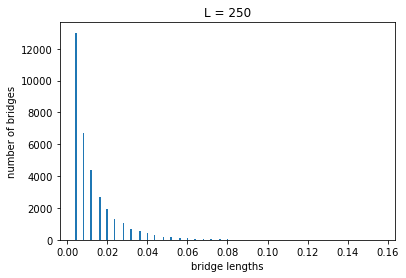
\includegraphics[width=\textwidth]{../images/bridge_lengths_L250.png} 
	\end{subfigure}
	\begin{subfigure}[t]{0.3\textwidth} 
		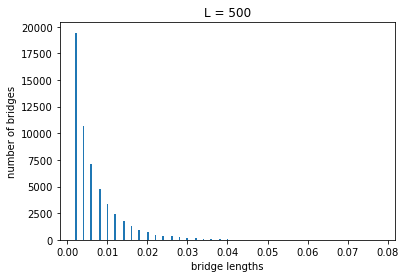
\includegraphics[width=\textwidth]{../images/bridge_lengths_L500.png} 
	\end{subfigure}
	\begin{subfigure}[t]{0.3\textwidth} 
		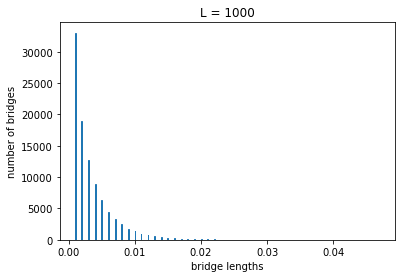
\includegraphics[width=\textwidth]{../images/bridge_lengths_L1000.png} 
	\end{subfigure}
	\caption{Распределение длин мостов.}
\end{figure}

\begin{figure}[H]
	\centering
	\begin{subfigure}[t]{0.3\textwidth} 
		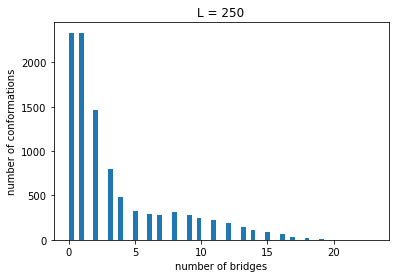
\includegraphics[width=\textwidth]{../images/bridges_count_L250.png} 
	\end{subfigure}
	\begin{subfigure}[t]{0.3\textwidth} 
		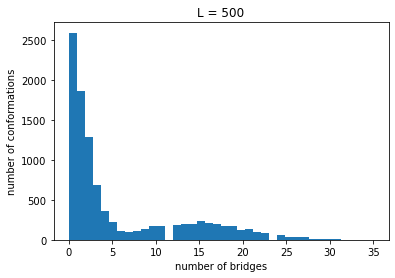
\includegraphics[width=\textwidth]{../images/bridges_count_L500.png} 
	\end{subfigure}
	\begin{subfigure}[t]{0.3\textwidth} 
		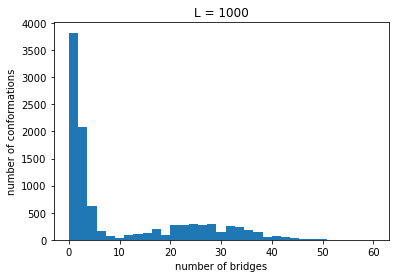
\includegraphics[width=\textwidth]{../images/bridges_count_L1000.png} 
	\end{subfigure}
	\caption{Распределение числа мостов в конформации.}
\end{figure}

\begin{figure}[H]
	\centering
	\begin{subfigure}[t]{0.3\textwidth} 
		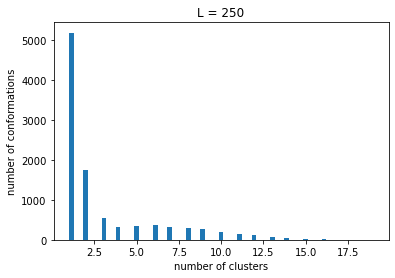
\includegraphics[width=\textwidth]{../images/clusters_count_L250.png} 
	\end{subfigure}
	\begin{subfigure}[t]{0.3\textwidth} 
		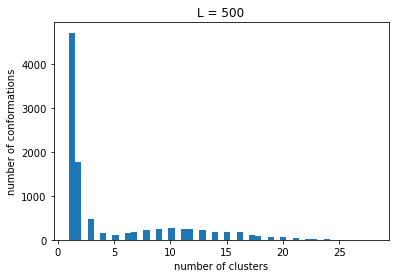
\includegraphics[width=\textwidth]{../images/clusters_count_L500.png} 
	\end{subfigure}
	\begin{subfigure}[t]{0.3\textwidth} 
		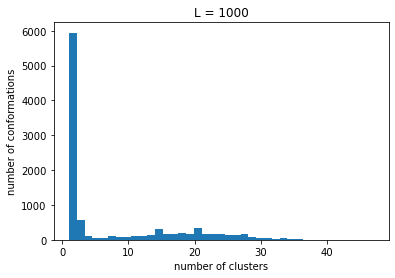
\includegraphics[width=\textwidth]{../images/clusters_count_L1000.png} 
	\end{subfigure}
	\caption{Распределение числа кластеров в конформации.}
\end{figure}

\begin{figure}[H]
	\centering
	\begin{subfigure}[t]{0.3\textwidth} 
		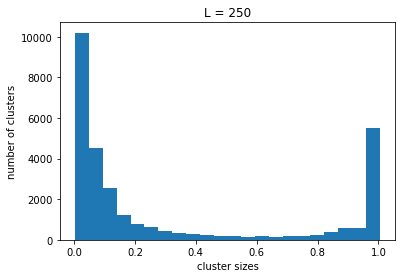
\includegraphics[width=\textwidth]{../images/cluster_sizes_L250.png} 
	\end{subfigure}
	\begin{subfigure}[t]{0.3\textwidth} 
		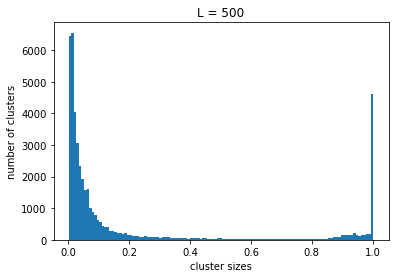
\includegraphics[width=\textwidth]{../images/cluster_sizes_L500.png} 
	\end{subfigure}
	\begin{subfigure}[t]{0.3\textwidth} 
		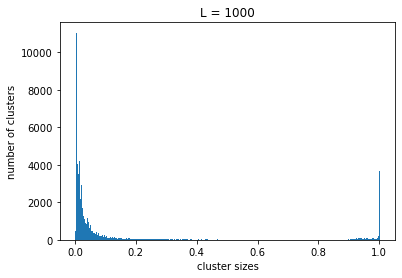
\includegraphics[width=\textwidth]{../images/cluster_sizes_L1000.png} 
	\end{subfigure}
	\caption{Распределение размера кластеров.}
\end{figure}

\begin{figure}[H]
	\centering
	\begin{subfigure}[t]{0.3\textwidth} 
		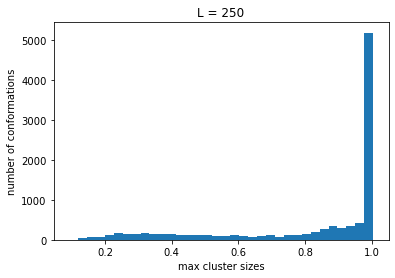
\includegraphics[width=\textwidth]{../images/max_cluster_size_L250.png} 
	\end{subfigure}
	\begin{subfigure}[t]{0.3\textwidth} 
		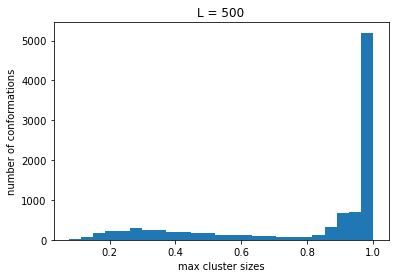
\includegraphics[width=\textwidth]{../images/max_cluster_size_L500.png} 
	\end{subfigure}
	\begin{subfigure}[t]{0.3\textwidth} 
		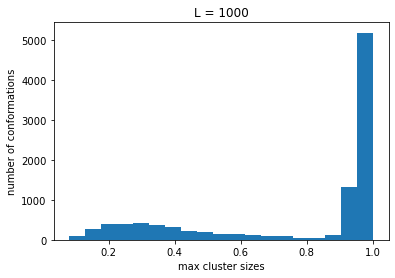
\includegraphics[width=\textwidth]{../images/max_cluster_size_L1000.png} 
	\end{subfigure}
	\caption{Распределение размера наибольшего кластера в конформации.}
\end{figure}


\subsection{Результаты разбиения на кластеры}
Результаты анализа связи между намагниченностью и количеством и размерами кластеров и мостов подтверждают сказанное выше. У конформаций с большим числом кластеров обычно намагниченность ниже чем у конформаций с одним большим кластером. 

Я рассмотрел несколько параметров: количество мостов, количество кластеров, суммарная длина мостов, размер наибольшего кластера. Наилучшим способом разделения конформаций на магнитные и немагнитные сейчас выглядит именно разделение по размеру наибольшего кластера. Как видно на рис.\ref{fig:mag_from_max_cluster} при разбиении по данному параметру разброс намагниченности значительно ниже, чем при разбиении по радиусу инерции. Данный параметр можно легко масштабировать для разных длин конформаций.

\begin{figure}[h]
	\centering
	\caption{График размера наибольшего кластера и квадрата намагниченности для 10000 конформаций длины 1000}
	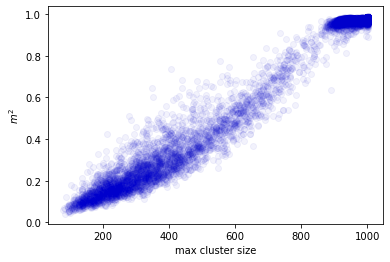
\includegraphics[width=0.8\textwidth]{../images/mag_from_cluster_size.png} 
	\label{fig:mag_from_max_cluster}
\end{figure}

\paragraph{Сравнение разделения по кластерам и по радиусу}
Чтобы оценить и сравнить эффективность разбиения конформаций при помощи размера наибольшего кластера и радиуса инерции воспользуемся следующим способом.

\begin{enumerate}
	\item Зададим значение намагниченности $\mu$, начиная с которого будем считать конформации намагниченными.
	\item Из всех сгенерированных конформаций возьмём $n$ конформаций с наименьшими радисоми инерции, и $n$ конформаций с наибольшими размерами кластеров.
	\item Среди выбранных конформаций посчитаем $k_{\mu, n}$ количество конформаций, намагниченность которых $< \mu$. Чем ниже это значение, тем лучше соответствующий способ разделения.
	\item Повторяем предыдущие пункты для разных значений $\mu$ и $n$.
\end{enumerate}

Сравнивая полученные значения $k_{\mu, n}$ можем определить, какой из способов эффективнее. На рис.\ref{fig:kmun_example} видно как примерно ведут себя данные значения: до определённого n они равны 0, затем, дойдя до границы между магнитными и немагнитными конформациями, оно начинает расти, после чего рост становится линейным, так как все оставшиеся конформации не являются магнитными. 
Лучше разницу между двумя способами видно на рис.\ref{fig:kmun_dif}, где, при всех значениях $\mu$ и $n$, разница $k_{\mu, n}$ остаётся отрицательной. То есть разделения по радиусу инерции всегда оставляет больше немагнитных конформаций, чем разделение по размеру кластеров.

\begin{figure}[h]
	\centering
	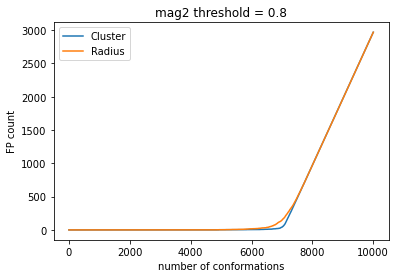
\includegraphics[width=0.6\textwidth]{../images/cluster_and_radius_mu0.8.png} 
	\caption{График $k_{\mu, n}$ для разделения по кластерам и по радиусу, при $\mu = 0.8$.}
	\label{fig:kmun_example}
\end{figure}

\begin{figure}[h]
	\centering
	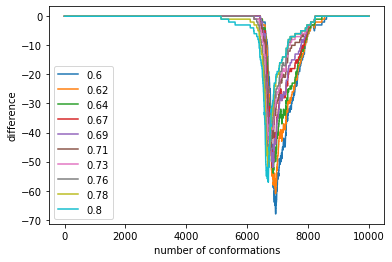
\includegraphics[width=0.6\textwidth]{../images/radius_and_cluster_comparising_L1000.png}
	\label{fig:kmun_dif}
	\caption{График разности: $k_{\mu, n}$ при кластерном разделении и $k_{\mu, n}$ при разделении по радиусам. На 10000 конформаций длины 1000. Каждая линия соответствует одному значению $\mu$.}
\end{figure}



\subsection{Кумулянт и точка перехода}

Кумулянт Биндера для одной реплики при заданной температуре вычисляется по формуле $U = 1 - \frac{\langle m^4\rangle}{3\langle m^2\rangle ^2}$. Дальше Значения усредняются между репликами при каждой температуре $\langle U\rangle = \frac{1}{n}\sum_{i=1}^{n}U_i$ 
Погрешность кумулянта от реплики к реплике вычисляется как среднеквадратичное отклонение по формуле $\sqrt{\frac{1}{n}\sum_{i=1}^{n}(\langle U\rangle - U_i)^2}$

Как видно на рис.\ref{fig:cumulant_raw} вычисление кумулянта на всех сгенерированных конформациях даёт слишком больше погрешности от конформации к конформации, из-за этого становится невозможно определить точку перехода.

\begin{figure}[h]
	\centering
	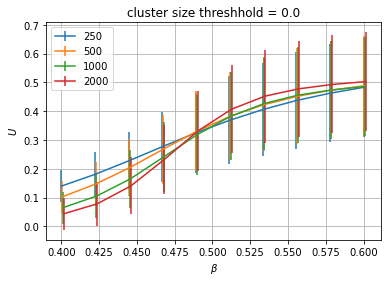
\includegraphics[width=0.5\textwidth]{../images/Cumulant_raw_beta0.4_0.6.png}
	\caption{кумулянты построенные на всех полученных конформациях}
	\label{fig:cumulant_raw}
\end{figure}

Описанный выше способ разделения конформаций на магнитные и немагнитные должен позволить уменьшить погрешность при вычислении кумулянта. Чтобы подобрать значение параметра(размер наибольшего кластера), при котором будет происходить разделение, мы стали перебирать значения, и следить за поведением точки пересечения. Предположительно при увеличении параметра точка пересечения должна двигаться в сторону нуля, и начиная с определённого значения она должна остановиться.

Точка пересечения в данном случае вычисляется путём генерации отрезков по точкам замеров: рядом с предполагаемой точкой пересечения берём несколько замеров, в них генерируем точки из нормального распределения, распределение построено по значению и погрешности кумулянта.


Эксперименты с разделением конформаций по радиусу инерции показали, что таким образом можно выделить наборы конформаций разных длин так, что для них будет возможно найти точку перехода.

\begin{figure}[h]
	\centering
	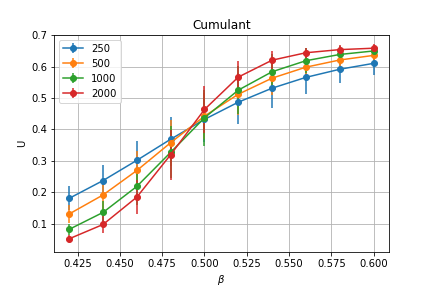
\includegraphics[width=1\textwidth]{../images/Cumulant_beta0.4_0.6.png} 
	\caption{Значения кумулянтов после отбора конформаций по радиусам инерции}
\end{figure}
